\documentclass[a4paper,10pt]{article}
\usepackage[utf8x]{inputenc}
\usepackage[serbian]{babel}

\usepackage[version=3]{mhchem} % Package for chemical equation typesetting
\usepackage[margin=2.5cm]{geometry}
\usepackage{pgfplots}
\usepackage{graphicx} % Required for the inclusion of images
\usepackage{natbib} % Required to change bibliography style to APA
\usepackage{amsmath} % Required for some math elements 
\usepackage{subfig} % For multiple figures side-by-side
\usepackage{url} % For linking url's properly

\setlength\parindent{0pt} % Removes all indentation from paragraphs

%\usepackage{times} % Uncomment to use the Times New Roman font

%----------------------------------------------------------------------------------------
%	DOCUMENT INFORMATION
%----------------------------------------------------------------------------------------

\title{OPNA: Drugi projektni zadatak \\ Šturmova teorema} % Title

\author{Aleksa \textsc{Ilić}} % Author name

\date{25. decembar 2020.} % Date for the report

\begin{document}

\maketitle % Insert the title, author and date

\begin{abstract}
    Rad prikazuje praktičnu realizaciju konzolnog programa koji izvršava numeričku procenu Šturmove teoreme sa arbitrarnom preciznošću i modularnošću ispisa
\end{abstract}

%----------------------------------------------------------------------------------------
%	SECTION: UVOD
%----------------------------------------------------------------------------------------

\section{Uvod}
\subsection{Opis problema}

Za zadati polinom $P(x)$ sa realnim koeficijentima nad segmentom $[a,b]$ odrediti:

\begin{enumerate}
    \item Euklidovim algoritmom najveći zajednički delilac $Q(x) = GCD(P(x), P'(x))$
    \item Za polinom $P(x) := P(x)/Q(x)$, upotrebom Šturmove teoreme, odrediti broj nula na $[a,b]$
    \item Neka je $k$ broj decimala na koji se zaokružuje neki relan broj. Za koeficijente polinoma
    \[P(x) = a_nx^n + a_{n-1}x^{n-1} + ... + a_1x + a_0\]
    sa realnim koeficijentima
    \[a_n,a_{n-1},...,a_1,a_0\]
    odrediti niz naniže zaokruženih koeficijenata
    \[\alpha_n,\alpha_{n-1},...,\alpha_1,\alpha_0\]
    određenih po sledećim pravilima:
    \begin{itemize}
        \item ako je $a_k = a_0.a_1 ... a_ka_{k+1} ... > 0$ tada $\alpha_k = a_0.a_1 ... a_k$
        \item ako je $a_k = a_0.a_1 ... a_ka_{k+1} ... < 0$ tada $\alpha_k = a_0.a_1 ... a'_k$
        \hfill \break
        gde je $a′k$ naviše zaokružena cifra (uz eventualno posledično zaokruživanje i prethodnih cifara za jedan broj naviše
    \end{itemize}
    Formirati polinom
    \[P(x) = \alpha_nx^n + \alpha_{n-1}x^{n-1} + ... + \alpha_1x + \alpha_0\]
\end{enumerate}

\subsection{Definicije}
\label{definitions}
\begin{description}
\item[Šturmova teorema:]
Neka je $P(x)$ polinom sa realnim koeficijentima koj razmatramo nad segmentom $[a,b]$ realne prave koji na segmentu može da ima samo jednostruke nule. Formirajmo niz polinoma $P_0,P_1,...,P_r$ na sledeći način:
\begin{enumerate}
    \item $P_0(x) = P(x)$
    \item $P_1(x) = P'(x)$
    \item $P_{i+1}(x) = -REM(P_i(x),P_{i-1}(x))$ za $i = 1,2,...,r-1; i_r(x) = C - Const.$
\end{enumerate}
Neka je $\xi \in [a,b]$, označimo:
\[V(\xi) \text{ broj promena znakova u nizu } P_0(\xi),P_1(\xi),...,P_r(\xi),\]
ignorišući eventualno javljanje nule u tom nizu. Tada razlika:
\[N = V(a) - V(b)\]
određuje broj nula polinoma $P(x)$ na segmentu $[a,b]$.
\end{description} 
 
%----------------------------------------------------------------------------------------
%	SECTION: OPIS REŠENJA
%----------------------------------------------------------------------------------------

\section{Opis rešenja}

Za realizaciju rešenja korišćen je programski jezik \textbf{C++17} zajedno sa najnovijom verzijom \textbf{Boost} biblioteka u trenutku pisanja ovog rada. Celokupan, dokumentovani izvorni kod dostupan je na autorovom github profilu \cite{WEBSITE:Github}.

\vspace{11pt}
Aktuelna verzija (v0.1.1) rešenja, sa podrazumevanim vrednostima veličine tipova, korišćena je za generisanje svih slika i računskih ispisa. Rešenje omogućava visoku preciznost pri numeričkom računu, a ona se može i dodatno povećati ukoliko korisnik to želi. Takođe, ispis rešenja je vrlo modularan te korisnik može, dodavanjem odgovarajućih prarametara, dobiti željeni ispis. Pregled svih parametara i podrazumevanih podešavanja dat je na Slici \ref{fig:version}. Parameter --gcd omogućava optimizaciju korišćenjem polinoma $P(x)$ nadevenim u koraku 2 opisa problema.

\begin{figure}[h]
\begin{center}
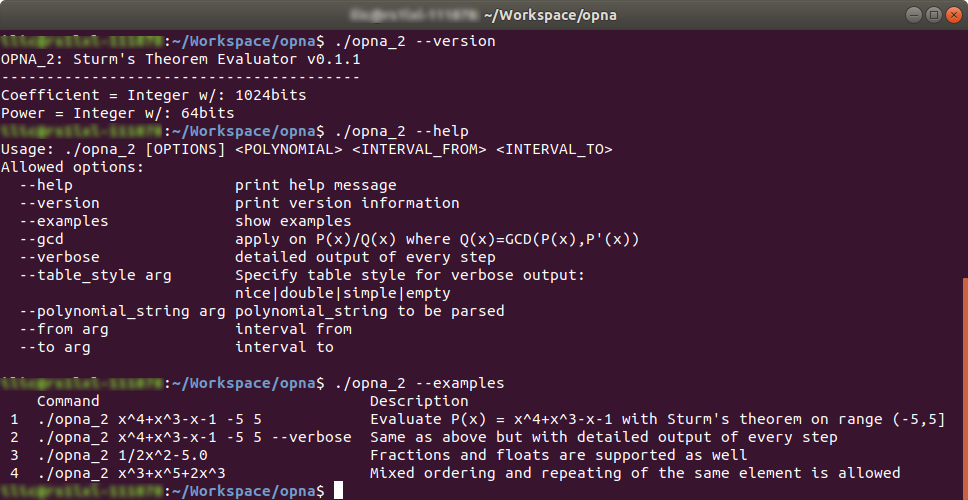
\includegraphics[width=0.9\textwidth]{version.png}
\caption{Podrazumevana podešavanja i pomoćni ekran}
\label{fig:version}
\end{center}
\end{figure}

\subsection{Primeri ispisa}

Na slikama \ref{fig:wikipedia_example1} i \ref{fig:wikipedia_example2} nalaze se primeri kojima se demonstrira program na primeru polinoma: 
\[P(x)=x^4+x^3-x-1\] 
Ideja autora je da ovim primerom prikaže modularne sposobnosti ispisa, te neće biti analize samog numeričkog računa. 
Prva slika prikazuje podrazumevani ispis, gde se prikazuje samo rešenje tj. broj realnih korena na itervalu, kao i detaljniji, ``verbose'', ispis koji prikazuje i međurezultate. Takođe je u ovom primeru promenjen podrazumvani stil tabele na ``nice''. Drugi primer prikazuje korišćenje optimizacionog ``--gcd'' parametra i njegov efekat na račun i ispis.

\begin{figure}
\begin{center}
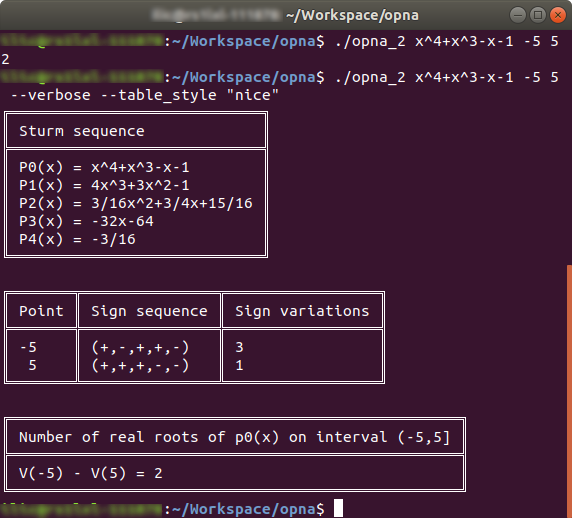
\includegraphics[width=0.75\textwidth]{wikipedia_example1.png}
\caption{Podrazumevani i ``verbose'' prikaza sa ``nice'' tabelarnim prikazom}
\label{fig:wikipedia_example1}
\end{center}
\end{figure}

\begin{figure}
\begin{center}
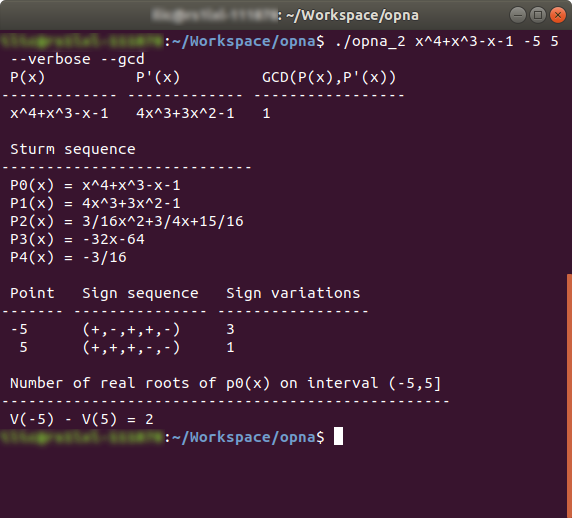
\includegraphics[width=0.75\textwidth]{wikipedia_example2.png}
\caption{``verbose'' prikaz sa ``gcd'' optimizacijom}
\label{fig:wikipedia_example2}
\end{center}
\end{figure}

\newpage

%----------------------------------------------------------------------------------------
%	SECTION: RAČUN
%----------------------------------------------------------------------------------------

\section{Izračunavanje polinoma}
Posmatrajmo funkciju:
\begin{equation}
    f(x) = (x+3)(x−2)^2(x+1)^3
\end{equation}Njen graf dat je ispod:
\begin{center}
\begin{tikzpicture}
\begin{axis}[
    extra y ticks = 0,
    extra y tick style  = { grid = major },
    axis lines = left,
    xlabel = $x$,
    ylabel = {$f(x)$},
    xmin=-3.5, xmax=3.5,
    ymin=-60, ymax=60
]
%Below the red parabola is defined
\addplot [
    samples=100, 
    color=red,
]
{x^6 + 2*x^5 - 8*x^4 - 14*x^3 + 11*x^2 + 28*x + 12};
\addlegendentry{$f(x)$}
\node[label={270:{(-3,0)}},circle,fill,inner sep=1pt] at (axis cs:-3,0) {};
\node[label={270:{(-1,0)}},circle,fill,inner sep=1pt] at (axis cs:-1,0) {};
\node[label={270:{(2,0)}},circle,fill,inner sep=1pt] at (axis cs:2,0) {};
\end{axis}
\end{tikzpicture}
\end{center}

Primetimo da na intervalu $[-3,3]$ data funkcija poseduje 3 realna korena, i to su redom: $-3, -1, 2$. Kako je data funkcija polinomijalna, mozemo razviti $f(x)$ do polinomnog oblika i dobiti $P(x)$ koji mozemo dalje koristiti u programu. Pa tako dobijamo
\begin{equation}
    P(x) = x^6 + 2x^5 - 8x^4 - 14x^3 + 11x^2 + 28x + 12
\end{equation}

\subsection{Podešavanja programa}
Za prikaz rešenja korišćene su podrazumevane veličine tipova. Korišćen je (``verbose'') režim ispisa uz ``simple'' stil tabela. Razmatrani interval je $(-5,5]$. 
Program je pokrenut dva puta, jednom uz upotrebu gorepomenutih podešavanja, i drugi put proširenjem podešavanja parametrom ``--gcd''. Razlog proširenja jeste prikaz optimizacije na realnom primeru.
\vspace{11pt}

Rezultati su izneti u tekstualnom formatu kao proizvod izvršenja realizovanog programa sa pomenutim parametrima. Autor se odlučio za takav prikaz jer omogućava veću fleksibilnost u odnosu na sliku terminalnog prozora ukoliko čitalac želi da rezultate prekopira i koristi u svojim istraživanjima. Autor garantuje da svi brojevi odgovaraju ispisu programa i nisu na bilo koji način menjani, ali su neke međuverižne aproksimacije isečene zarad lepšeg ispisa.

\subsection{Rezultati}
\begin{verbatim}
./opna_2 x^6+2x^5-8x^4-14x^3+11x^2+28x+12 -5 5 --verbose
 Sturm sequence                              
---------------------------------------------
 P0(x) = x^6+2x^5-8x^4-14x^3+11x^2+28x+12    
 P1(x) = 6x^5+10x^4-32x^3-42x^2+22x+28       
 P2(x) = 29/9x^4+47/9x^3-29/3x^2-199/9x-94/9 
 P3(x) = 12150/841x^3-36450/841x-24300/841   

 Point   Sign sequence   Sign variations 
------- --------------- -----------------
 -5      (+,-,+,-)       3               
  5      (+,+,+,+)       0               

 Number of real roots of P0(x) on interval (-5,5] 
--------------------------------------------------
 V(-5) - V(5) = 3                                 
\end{verbatim}

\begin{verbatim}
./opna_2 x^6+2x^5-8x^4-14x^3+11x^2+28x+12 -5 5 --verbose --gcd
 P(x)                               P'(x)                           GCD(P(x),P'(x)) 
---------------------------------- ------------------------------- -----------------
 x^6+2x^5-8x^4-14x^3+11x^2+28x+12   6x^5+10x^4-32x^3-42x^2+22x+28   -x^3+3x+2       

 Sturm sequence         
------------------------
 P0(x) = -x^3-2x^2+5x+6 
 P1(x) = -3x^2-4x+5     
 P2(x) = -38/9x-44/9    
 P3(x) = -2025/361      

 Point   Sign sequence   Sign variations 
------- --------------- -----------------
 -5      (+,-,+,-)       3               
  5      (-,-,-,-)       0               

 Number of real roots of P0(x) on interval (-5,5] 
--------------------------------------------------
 V(-5) - V(5) = 3                                 
\end{verbatim}
%----------------------------------------------------------------------------------------
%	SECTION: DISKUSIJA
%----------------------------------------------------------------------------------------

\section{Diskusija rezultata}

Program je kroz 4 iteracije, u oba slučaja, došao do broja koji odgovara iznetom očekivanju na početku poglavlja 3. Primetimo da je u drugom slučaju, kada se koristi GCD optimizacija tj. 
$P(x) := \frac{P(x)}{GCD(P(x),P'(x))}$, 
iako je rezultat sračunat iz istog broj iteracija, sekvenca polinoma koja se dobija jako pogodnija za pisanje i numeričku analizu.

%----------------------------------------------------------------------------------------
%	BIBLIOGRAPHY
%----------------------------------------------------------------------------------------

\bibliographystyle{apalike}

\bibliography{sample}

%----------------------------------------------------------------------------------------


\end{document}